\subsection{Commit Analyzer Plug-ins}
\label{sec:CommitAnalyzerPlugins}
\ToDo{
\begin{itemize}
	\item Definition and usage of plug-in-specific configuration parameters in introduction of parent section?
	\item Purpose of plug-in type
	\item Typical input
	\item Realization via implementation of abstract class along example
	\begin{itemize}
		\item Processing data model element instances
		\item Storing results
	\end{itemize}
\end{itemize}

% Detailed outline/steps
1.	New plain Java project
	a.	Name = CommitAnalyzer
	b.	Execution environment JRE = JavaSE-1.8 or higher
2.	Add ComAnI infrastructure plug-in to Java Build Path, in Eclipse
	a.	Right click on project “CommitAnalyzer”
	b.	Select “Properties”
	c.	Select “Java Build Path”
	d.	Select “Libraries” tab
	e.	Click “Add External JARs...”
	f.	Select the “ComAnI.jar” file from where you extracted it and click “Open”
	g.	Close properties dialog by clicking “Ok”.
3.	New package “core” will contain analyzer main class
4.	New Java class “CommitAnalyzer”
5.	This class must extend the AbstractCommitAnalyzer class
	a.	Import net.ssehub.comani.analysis.AbstractCommitAnalyzer;
	b.	Add required constructor
	c.	Add required methods
6.	Implement algorithms for the different methods; custom classes can be created and used as well. It is only import to know the main class subclassing the AbstractCommitAnalyzer as we need this later for instance definition in the ComAnI configuration file.
7.	Export the final commit analyzer as “JAR file” (not a runnable!), in Eclipse
	a.	Right click on project “CommitAnalyzer”
	b.	Select “Export”
	c.	Select “JAR file” under “Java” directory and click “Next”
	d.	Only export the “src” directory, in particular, do not include the “ComAnI.jar”
	e.	Save the JAR file to any location, but note that it has to be in the plug-ins directory specified in the ComAnI configuration file for later use
	f.	Click “Finish”
8.	For using it, copy the created JAR file to the ComAnI plug-ins directory and specify the analyzer via its fully qualified main class name as the desired analyzer in the configuration file. In our example, this looks like: analysis.analyzer = core.CommitAnalyzer

As an alternative to step 2: If the ComAnI infrastructure project is in place, you may also include the project as a dependency to the Java Build Path. The rest is the same as above.

Custom properties need to start with analysis.*. Otherwise they will not be available as part of the properties object passed to the analyzer as constructor parameter. Using custom parameters is as simple as scanning the received properties object for the key, the analyzer expects and then reading the value and processing/configuring the analyzer as desired. Such properties should be made public and have description how to define and use them. The infrastructure takes care of reading the configuration file also with the new properties and passing it the analyzer as long as it conforms to the naming convention (starts with analysis.*).
}

\begin{figure}[ht] % t für top, b = bottom, h = here
	\centering
		%trim={<left> <lower> <right> <upper>}
		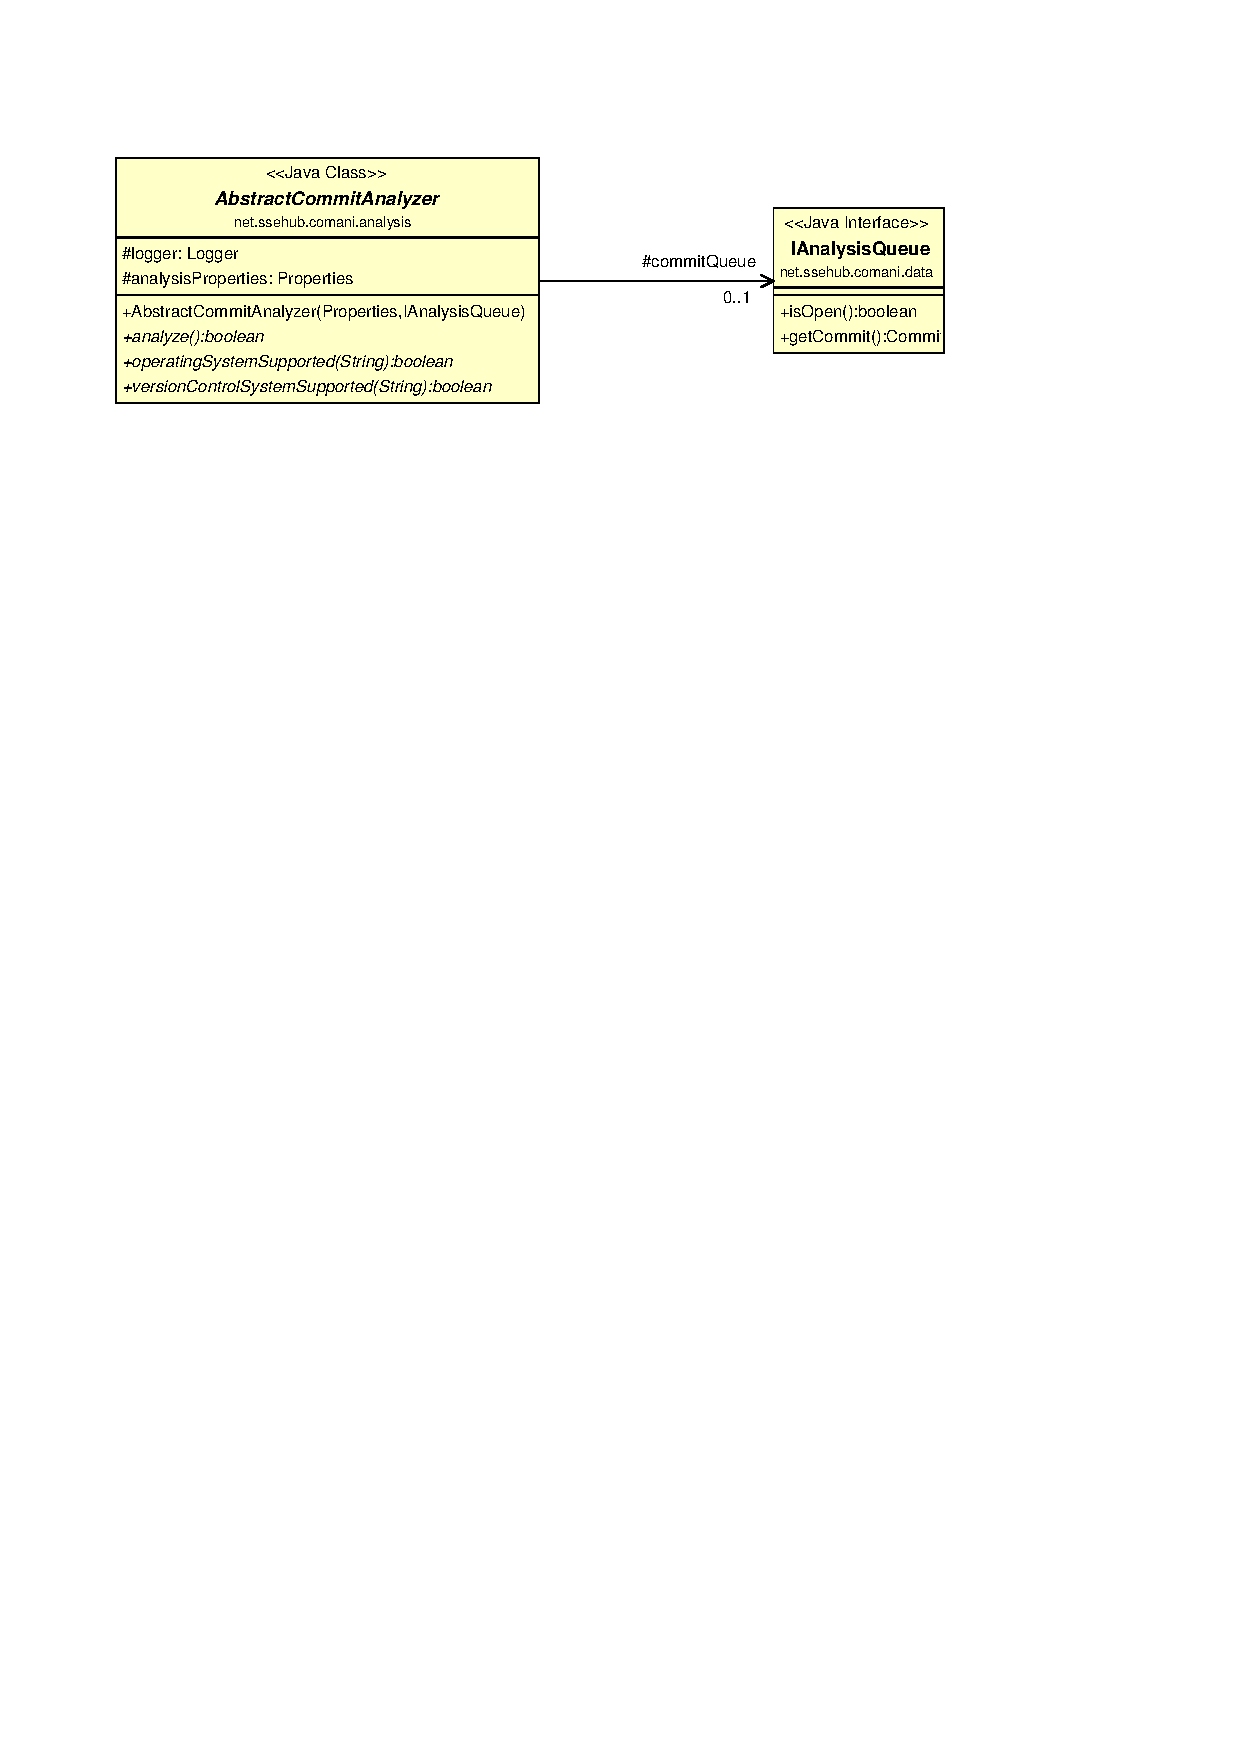
\includegraphics[width=\columnwidth,trim={1,9cm 22,8cm 5cm 2,6cm},clip]{inserts/comani_abstract_commit_analyzer.pdf}
  \caption{\thetool{} \texttt{AbstractCommitAnalyzer} class}
	\label{fig:AbstractCommitAnalyzerClass}
\end{figure}

\begin{figure}[ht]
	\centering
		\lstinputlisting[caption={Blueprint of a \thetool{} commit analyzer main class},label=lst:CommitAnalyzerBlueprint,basicstyle=\small,language=Java]{inserts/CommitAnalyzer.java}
\end{figure}